\documentclass[conference]{IEEEtran}

\IEEEoverridecommandlockouts
% The preceding line is only needed to identify funding in the first footnote. If that is unneeded, please comment it out.
\usepackage{fancyhdr}
\usepackage{cite}
\usepackage{amsmath,amssymb,amsfonts}
\usepackage{algorithmic}
\usepackage{graphicx}
\usepackage{textcomp}
\usepackage{xcolor}
\usepackage{subcaption}
\usepackage{blindtext}
\usepackage{microtype}
\usepackage{booktabs}
\usepackage{caption}
\usepackage[numbers,sort&compress]{natbib}
\usepackage{algorithm}
\usepackage{algpseudocode}
\def\BibTeX{{\rm B\kern-.05em{\sc i\kern-.025em b}\kern-.08em

    T\kern-.1667em\lower.7ex\hbox{E}\kern-.125emX}}
\begin{document}

% Create custom colour for text highlighting
\definecolor{twblue}{HTML}{1f497d}
\definecolor{structure}{HTML}{1f497d}
\definecolor{blindtext}{HTML}{D3D3D3}

\pagestyle{fancy}
\fancyhf{}
\rfoot{\thepage} % Seitenzahl im rechten Fuß

\title{ EVALUATING MODEL PREDICTIVE CONTROL IN DIFFERENTIAL DRIVE ROBOTICS: \\ COMPREHENSIVE LITERATURE REVIEW }

\author{\IEEEauthorblockN{\textbf{Student:} Eppacher Kevin, BSc. \textbf{PK:} 2310331013}
        \IEEEauthorblockN{\textbf{Peer ReviewerIn:} Schweiger Simon, MSc.}
}


\maketitle
%%%%%%%%%%%%%%%%%%%%%%%%%%%%%%%%%%%%%%%%%%%%%%%%%%%%%%%%%%%%%%%%%%

\begin{abstract}
    Mobile robots are widely used in industries, households, and public spaces, such as Autonomous
    Mobile Robots (AMRs) for transporting goods in intralogistics, vacuum/mower robots, and service
    robots in restaurants. However, mobile robots face several challenges, including highly dynamic
    environments, external disturbances such as slippage, which can complicate localization over 
    long distances, and other environmental factors. The goal of this work is to develop a system that 
    enables a mobile robot to navigate optimally and collision-free. Several established approaches,
    such as the Dynamic Window Approach (DWA) and Move Base Flex, have already proven effective.
    The Dynamic Window Approach limits the robot's velocity space to ensure collision avoidance, while
    Move Base Flex provides a flexible interface for path planning and execution, allowing for the 
    integration of different navigation frameworks. In this work, a control system is developed for 
    dynamic obstacle avoidance using a nonlinear Model Predictive Controller (nMPC). The results are 
    compared with the well-established Move Base DWA from ROS1. Both controllers are evaluated in a 
    Gazebo simulation under three conditions: with static objects, with dynamically detected obstacles, 
    and without obstacle avoidance (i.e., without laser scan).

    (Results will follow...)
\end{abstract}

\begin{IEEEkeywords}
Model Predictive Control, Differential Drive Robots, Obstacle Avoidance, Autonomous Mobile Robots, Control Algorithms
\end{IEEEkeywords}

%%%%%%%%%%%%%%%%%%%%%%%%%%%%%%%%%%%%%%%%%%%%%%%%%%%%%%%%%%%%%%%%%%
\section{Introduction}
% Introduction to the paper’s main subject (subject = lokale Pfadplanung)

Mobile robots are becoming increasingly indispensable in various fields such as intralogistics, public, and private services, with applications ranging from autonomous floor-cleaning robots to vacuum cleaners. In dynamic environments, these robots are frequently confronted with fast-moving obstacles, which they must detect and avoid in real-time. The conventional approach to navigation involves the mobile robot first creating a map of its surroundings, typically using an occupancy grid to store information about static objects such as walls. Based on this map, a global path is planned using algorithms such as Rapidly Exploring Random Tree (RRT), which the robot subsequently follows \cite{thrun2005probabilistic}.

However, it is important to note that while the global path provides an initial route, it is updated at a lower frequency compared to the local planner, which operates at a higher update rate. The local planner is responsible for adjusting the robot's trajectory in real-time to avoid newly detected obstacles, while still adhering to the waypoints of the global path \cite{siegwart2011autonomous}. This separation between global path planning and local obstacle avoidance is critical in ensuring that the robot can navigate effectively in both known and dynamic environments \cite{khatib1986real}.

% Motivation for creating paper contribution (sehr grobe Übersicht über sota)

\cite{ASAP} conducted a comprehensive comparison of its developed local planner, ASAP, with other seminal planners, including DWA, TEB, and MPC. In Figure \ref{fig:DWA_TEB_MPC_ASAP_path}, the performance of these planners is compared as they guide a mobile robot to follow a global path while avoiding obstacles. 

\begin{figure}[!h]
    \centering
    \includegraphics[width=1\columnwidth]{images/DWA_TEB_MPC_ASAP_path.png}
    \caption{Blockdiagram of nMPC for future Implementation }
    \label{fig:DWA_TEB_MPC_ASAP_path}
\end{figure}

In this study, \cite{ASAP} evaluated the local planners based on metrics such as arrival time, cross track error, and computation time. 

\begin{figure}[!h]
    \centering
    \includegraphics[width=1\columnwidth]{images/DWA_TEB_MPC_ASAP_stats.png}
    \caption{Blockdiagram of nMPC for future Implementation }
    \label{fig:DWA_TEB_MPC_ASAP_stats}
\end{figure}

The findings in Figure \ref{fig:DWA_TEB_MPC_ASAP_stats} indicate that the MPC local planner achieved the shortest arrival time, while maintaining the same cross track error as the ASAP planner. However, when it comes to computation time, the ASAP controller was the fastest, with a processing time of just 0.2 ms, compared to DWA's 40 ms, TEB's 5 ms, and MPC's 18 ms. Furthermore, \cite{ASAP} highlights that the DWA planner had the highest collision rate, which also corresponds to its longer arrival time.

Similarly, \cite{MPCvsTEB} performed a comparison between MPC and TEB planners. The study evaluated both the TEB planner and various forms of MPC in terms of arrival time, path length, control effort, and CPU time. The results indicated that the TEB planner and the quadratic form of MPC had comparable arrival times, around 126.9 seconds. However, the time-optimal MPC, which is specifically optimized for minimizing arrival time, completed the task in just 116 seconds. In terms of path length and control effort, both planners showed similar performance. However, the computational time for MPC was found to be three times higher than that of the TEB planner, demonstrating the trade-off between efficiency and computational cost.

% Problem description arising from motivation (was fehlt im aktuellen sota -> vermeidung dynamischer Objekte)
\cite{ASAP} and \cite{MPCvsTEB} illustrate promising results for the MPC as local planner, especially due to the high adaptability forming the cost function for the required needs and the model adaptability, as for example omni-drive-directional-wheels. However, it is shown, that the MPC planner in combination with dynamic obstacle avoidance lack in computation time.

% Paper contribution
This work contributes to the state-of-the-art development, of a nonlinear Model Predictive Controller for a mobile robot with integrated dynamic obstacle avoidance. 

The main objective is to design a local planner that effectively addresses the challenges of dynamic obstacle avoidance, offering improved performance in real-time navigation within dynamic environments.

This work addresses these challenges by developing a nonlinear Model Predictive Controller (nMPC) for differential drive mobile robots, specifically designed for dynamic obstacle avoidance. The primary contribution is the integration of nMPC to improve real-time navigation performance in dynamic environments. Unlike conventional approaches such as DWA, the proposed nMPC effectively handles nonlinear dynamics and dynamic obstacles, offering superior prediction accuracy and responsiveness.

This paper contributes to the field by rigorously evaluating the nMPC against both DWA and recent advancements in local planning algorithms from the past five years. The results demonstrate that the nMPC provides enhanced trajectory optimization and obstacle avoidance capabilities, filling a crucial gap in mobile robot control by addressing scenarios that existing methods have not sufficiently solved.

% Paper structure
The rest of the paper is organized as follows: Section II discusses related work in local path planning and obstacle avoidance. Section III outlines the methodology used for our comparative evaluation. Section IV presents the results of simulations, and Section V concludes with a summary of findings and potential future research directions.


%%%%%%%%%%%%%%%%%%%%%%%%%%%%%%%%%%%%%%%%%%%%%%%%%%%%%%%%%%%%%%%%%%
\section{State-of-the-Art}

In this section, we provide an overview of several state-of-the-art local planners, including the Dynamic Window Approach (DWA), Timed Elastic Band (TEB), Model Predictive Control (MPC), Move Base Flex (MBF), Agile and Safe Pursuit (ASAP), and Reinforcement Learning (RL)-based planners. We explain how these planners function and highlight their key limitations, especially when operating in dynamic environments. Additionally, we discuss how nonlinear Model Predictive Control (nMPC) addresses these limitations and provides improved performance.

\subsection{Dynamic Window Approach (DWA)}
DWA is a popular local planner that selects safe and feasible velocities by sampling translational \((v)\) and rotational \((\omega)\) velocities within a dynamic window. These sampled velocities are evaluated through an objective function that balances forward movement and obstacle avoidance. DWA computes a set of trajectories and selects the one that maximizes progress toward the goal while ensuring the robot avoids collisions.

The velocities \(v\) and \(\omega\) are constrained within bounds, as shown in Equation \eqref{eq:dwa_constraints}:

\begin{equation}
\label{eq:dwa_constraints}
v_{min} \leq v \leq v_{max}, \quad \omega_{min} \leq \omega \leq \omega_{max}
\end{equation}

The objective function \(G(v, \omega)\) evaluates the alignment with the goal, distance to obstacles, and forward velocity, as described in Equation \eqref{eq:dwa_objective}:

\begin{equation}
\label{eq:dwa_objective}
G(v, \omega) = \alpha \cdot \text{heading}(v, \omega) + \beta \cdot \text{clearance}(v, \omega) + \gamma \cdot v
\end{equation}

While DWA is efficient and handles real-time obstacle avoidance well, it struggles with dynamic obstacles due to its lack of future obstacle movement prediction. The extensive velocity sampling can lead to increased computation times in complex environments.

Recent enhancements to DWA focus on improving computational efficiency and addressing the limitations in dynamic environments. A faster implementation of DWA based on non-discrete path representation \cite{lin2023faster} reduces the computational complexity by eliminating discrete path representations and employing polar coordinate transformations. Another improved version integrates reinforcement learning (RL) techniques \cite{zhou2022improved}, dynamically adjusting the sampling window size to better handle obstacles in real-time, which improves efficiency and accuracy in dynamic environments.

\subsection{Timed Elastic Band (TEB)}
TEB models the robot’s trajectory as a dynamic band that adjusts to avoid obstacles while satisfying kinodynamic constraints. The trajectory is continuously optimized using a cost function that takes into account the goal, collisions, and system dynamics.

The cost function \(J(\mathbf{x}, \mathbf{v})\) over the series of poses \(\mathbf{x}\) and velocities \(\mathbf{v}\) is defined in Equation \eqref{eq:teb_cost}:

\begin{equation}
\label{eq:teb_cost}
J(\mathbf{x}, \mathbf{v}) = \sum_{i=1}^{n-1} \left( \text{cost}_{\text{goal}}(x_i) + \text{cost}_{\text{collision}}(x_i) + \text{cost}_{\text{kinodynamics}}(v_i) \right)
\end{equation}

TEB is effective at generating smooth trajectories that adapt to obstacles and kinodynamic constraints. However, in highly dynamic environments, TEB's computational complexity can increase significantly. Additionally, its performance is sensitive to initial conditions and parameter tuning.

Recent improvements to TEB incorporate dynamic obstacle velocities using Kalman filtering to predict obstacle movement and optimize the trajectory in real time. This improved TEB method \cite{chen2021dynamic} enhances real-time performance by reducing the overall computational burden while maintaining a high success rate for dynamic obstacle avoidance.

\subsection{Model Predictive Control (MPC)}
MPC computes optimal control inputs over a prediction horizon by solving an optimization problem that accounts for both system dynamics and environmental constraints. Given the system model \(x_{k+1} = f(x_k, u_k)\), MPC minimizes the cost function defined in Equation \eqref{eq:mpc_cost}:

\begin{equation}
\min_{\vec{u}_k} J(\vec{x}_k, \vec{u}_k) = \phi(\vec{x}(N)) + \sum_{k=0}^{N-1} L(\vec{x}(k), \vec{u}(k))
\end{equation}

MPC offers smooth, optimized control over nonlinear dynamics, making it ideal for complex environments. However, it is computationally demanding, especially in real-time applications. Additionally, MPC requires highly accurate models of the robot and environment, which may not always be feasible in dynamic situations.

\subsection{Move Base Flex (MBF)}
MBF is a flexible framework in ROS that enables the integration of multiple global and local planners. It provides interfaces for different types of planners, recovery behaviors, and global path planning. The performance of MBF is dependent on the planners it integrates, and while it offers modularity, its capabilities in dynamic environments are inherited from the chosen planners (e.g., DWA, TEB).

MBF provides great flexibility but may suffer from the limitations of the specific planners it incorporates, such as limited performance in dynamic environments with fast-moving obstacles.

\subsection{Agile and Safe Pursuit (ASAP)}
ASAP uses pursuit-based control combined with safety constraints, allowing the robot to track a path while maintaining agility and avoiding obstacles. The control law minimizes the error between the robot’s current position and the pursuit point \(P(t)\) on the path, as defined in Equation \eqref{eq:asap_control}:

\begin{equation}
\label{eq:asap_control}
u(t) = \text{argmin} \| x(t) - P(t) \|
\end{equation}

With the safety constraint shown in Equation \eqref{eq:asap_safety}:

\begin{equation}
\label{eq:asap_safety}
\| P(t) - x_{\text{obs}}(t) \| \geq d_{\text{safe}}
\end{equation}

ASAP provides fast and agile movement while maintaining safety, but it struggles with complex nonlinear dynamics and requires careful tuning of the safety constraints to avoid overly conservative behavior.

\subsection{Reinforcement Learning (RL)-based Planners}
In recent years, RL-based planners have gained significant attention due to their ability to learn optimal behaviors in dynamic and complex environments. These planners do not rely on explicit models but instead learn from trial and error by interacting with the environment. RL-based planners can adapt to new environments, making them highly effective for dynamic obstacle avoidance.

However, RL-based planners face challenges in real-time applications due to the extensive training time required and the need for vast amounts of data. Additionally, their performance can be inconsistent if the training environment does not closely resemble the real-world application. Despite these challenges, RL-based planners show promise in handling complex scenarios where traditional model-based planners fall short.

\subsection{Advantages of Nonlinear Model Predictive Control (nMPC)}
nMPC addresses the shortcomings of traditional local planners by predicting future obstacle movements and directly incorporating the nonlinear dynamics of the robot. It optimizes the control inputs over a finite prediction horizon, ensuring that the robot can navigate dynamically changing environments with greater efficiency and precision.

Compared to DWA, TEB, MPC, and RL-based planners, nMPC offers improved handling of dynamic obstacles by continuously adjusting the robot's trajectory in real-time, optimizing for both safety and performance. It also handles nonlinear dynamics more effectively, making it a robust solution for highly dynamic environments.

%%%%%%%%%%%%%%%%%%%%%%%%%%%%%%%%%%%%%%%%%%%%%%%%%%%%%%%%%%%%%%%%%%
\section{Methods}

\begin{figure}[!h]
    \centering
    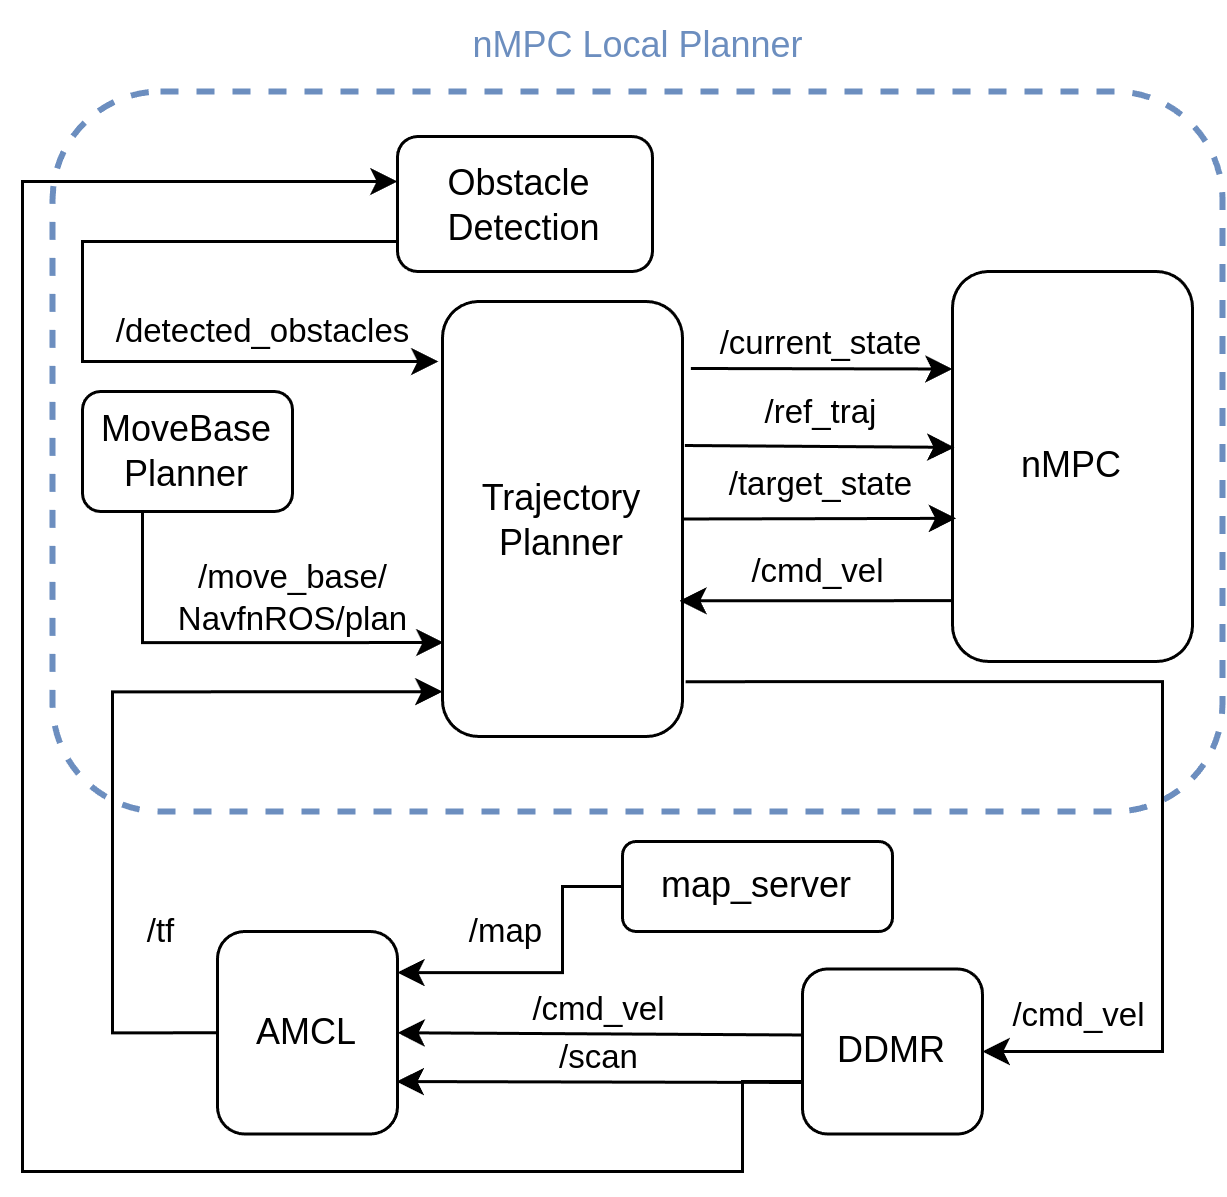
\includegraphics[width=1\columnwidth]{images/nMPC_Local_Planner_Diagram_2.png}
    \caption{ }
    \label{fig:nMPC_Local_Planner_Diagram_2}
\end{figure}


\subsection{nMPC}

\begin{figure}[!h]
    \centering
    \includegraphics[width=1\columnwidth]{images/MPC_Blockdiagram_Implementation.png}
    \caption{Blockdiagram of nMPC for future Implementation }
    \label{fig:MPC_Blockdiagram_Implementation}
\end{figure}

\begin{equation}\label{eq:state_vector}
    \mathbf{x} = \begin{bmatrix} x & y & \theta \end{bmatrix}^T
\end{equation}

\begin{equation}\label{eq:control_vector}
    u = \begin{bmatrix}
    v & \omega
\end{bmatrix}^T
\end{equation}


\begin{equation}
\label{eq:L_function}
\begin{aligned}
\min_{\vec{u}_k} J(\vec{x}_k, \vec{u}_k) = \phi(\vec{x}(N)) + \sum_{k}^{k+N-1} &
(\vec{x}_{R,k} - \vec{x}_{\text{ref},k})^T Q (\vec{x}_{R,k} - \vec{x}_{\text{ref},k}) \\
&+ \vec{u}_k^T R \vec{u}_k
\end{aligned}
\end{equation}

\begin{align}
\text{subject to: } \quad \vec{x}(k+1) &= f(\vec{x}(k), \vec{u}(k)), \\
\vec{x}(0) &= \vec{x}_0, \\
\vec{u}(k) &\in U, \quad \forall k \in [0, N-1], \\
\vec{x}(k) &\in X, \quad \forall k \in [0, N].
\end{align}


\begin{equation}
\label{eq:phi_definition}
\phi(\vec{x}(N)) = \frac{1}{2} \vec{x}_N^T S \vec{x}_N
\end{equation}

\begin{equation}
\label{eq:u_constraints}
\vec{u}_{\text{min}} \leq \vec{u}_k \leq \vec{u}_{\text{max}}, \quad \forall k \quad \text{…} \quad \vec{u} \in \mathbb{R}^2
\end{equation}

\begin{equation} \label{eq:1}
    x_{k+1} = Ax_k + Bu_k
\end{equation}


\begin{equation} \label{eq:discrete_state_space_equation_DDMR}
\begin{bmatrix}
    x_{k+1} \\
    y_{k+1} \\
    \theta_{k+1}
\end{bmatrix}
=
\begin{bmatrix}
    x_k \\
    y_k \\
    \theta_k
\end{bmatrix}
+ \Delta T
\begin{bmatrix}
    \cos(\theta) & 0 \\
    \sin(\theta) & 0 \\
    0 & 1
\end{bmatrix}
u_k
\end{equation}


\begin{equation}
\label{eq:collision_condition}
-\sqrt{(x_R - x_{\text{obst}})^2 + (y_R - y_{\text{obst}})^2} + (r_R + r_{\text{obst}}) \leq 0
\end{equation}









\subsection{Trajectory Planner}

\begin{algorithm}
\caption{Trajectory Interpolation}
\begin{algorithmic}[1]
\REQUIRE $P = \{(x_i, y_i, \text{yaw}_i)\}$, $d_{\text{pred}}$, $N$, $v_{\text{max}}$, $\alpha$
\ENSURE $P_{\text{new}}$, $T$
\STATE $D_i = \sum \sqrt{(x_{i+1} - x_i)^2 + (y_{i+1} - y_i)^2}$
\STATE Retain points where $D_i \leq d_{\text{pred}}$
\STATE $d_{\text{point}} = \frac{d_{\text{pred}}}{N}$
\STATE $T = \frac{d_{\text{point}}}{v_{\text{max}}}$
\STATE $T = T \cdot \alpha$
\STATE Interpolate $x$, $y$, and $\text{yaw}$ to get $N$ points
\RETURN $P_{\text{new}}$, $T$
\end{algorithmic}
\end{algorithm}




\begin{figure}[!h]
    \centering
    \includegraphics[width=1\columnwidth]{images/Interpolated_Trajectories.png}
    \caption{ }
    \label{fig:nMPC_16_vs_DWA_12_vs_TEB_6_Path}
\end{figure}


\begin{algorithm}
\caption{Filtered Obstacle Detection}
\begin{algorithmic}[1]
\STATE Filter laser scan data $(r_i, \theta_i)$ using:
\[
r_i < r_{\text{search}} \quad \text{and} \quad \left( -\frac{\theta_{\text{search}}}{2} \leq \theta_i \leq \frac{\theta_{\text{search}}}{2} \right)
\]
\STATE Convert filtered data to 2D coordinates:
\[
x_i = r_i \cos(\theta_i), \quad y_i = r_i \sin(\theta_i)
\]
\STATE Create lidar image:
\[
x_{\text{img}} = \left( \frac{x_i}{r_{\text{max}}} \times I_{\text{size}} \right) + \frac{I_{\text{size}}}{2}, \quad y_{\text{img}} = \left( \frac{y_i}{r_{\text{max}}} \times I_{\text{size}} \right) + \frac{I_{\text{size}}}{2}
\]
\STATE Apply Gaussian blur:
\[
I_{\text{blur}}(x, y) = \frac{1}{2\pi \sigma^2} \exp\left(-\frac{x^2 + y^2}{2\sigma^2}\right) \otimes I_{\text{img}}(x, y)
\]
\STATE Detect corners using Shi-Tomasi:
\[
\{(x_{\text{corner}}, y_{\text{corner}})\} = \text{Shi-Tomasi}(I_{\text{blur}})
\]
\STATE Sort by distance:
\[
d_i = \sqrt{x_{\text{corner}}^2 + y_{\text{corner}}^2}
\]
\STATE Transform detected corners into the robot frame:
\[
x_{\text{trans}} = x_{\text{robot}} + (x_{\text{corner}} \cos(\text{yaw}) - y_{\text{corner}} \sin(\text{yaw}))
\]
\[
y_{\text{trans}} = y_{\text{robot}} + (x_{\text{corner}} \sin(\text{yaw}) + y_{\text{corner}} \cos(\text{yaw}))
\]
\STATE Select $N_{\text{max}}$ closest points
\RETURN $(x_{\text{trans}}, y_{\text{trans}}, r_{\text{corner}})$ to nMPC
\end{algorithmic}
\end{algorithm}



%%%%%%%%%%%%%%%%%%%%%%%%%%%%%%%%%%%%%%%%%%%%%%%%%%%%%%%%%%%%%%%%%%
\section{Implementation Detail}

The experiments were conducted on a system equipped with an AMD Ryzen 5 7600X 6-Core Processor running at a maximum clock speed of 5.45 GHz. The system has 12 logical CPUs (2 threads per core) and 30 GB of RAM, with no swap space configured.

The experiments ran inside a Docker container, which utilized up to 4.808 GB of RAM (approximately 15.78 \% of the available memory) and had a peak CPU usage of 855.20 \%, indicating multi-core processing. The container handled a maximum of 393 processes during the experiments.

%%%%%%%%%%%%%%%%%%%%%%%%%%%%%%%%%%%%%%%%%%%%%%%%%%%%%%%%%%%%%%%%%%
\section{Discussion and Results}

\begin{figure}[!h]
    \centering
    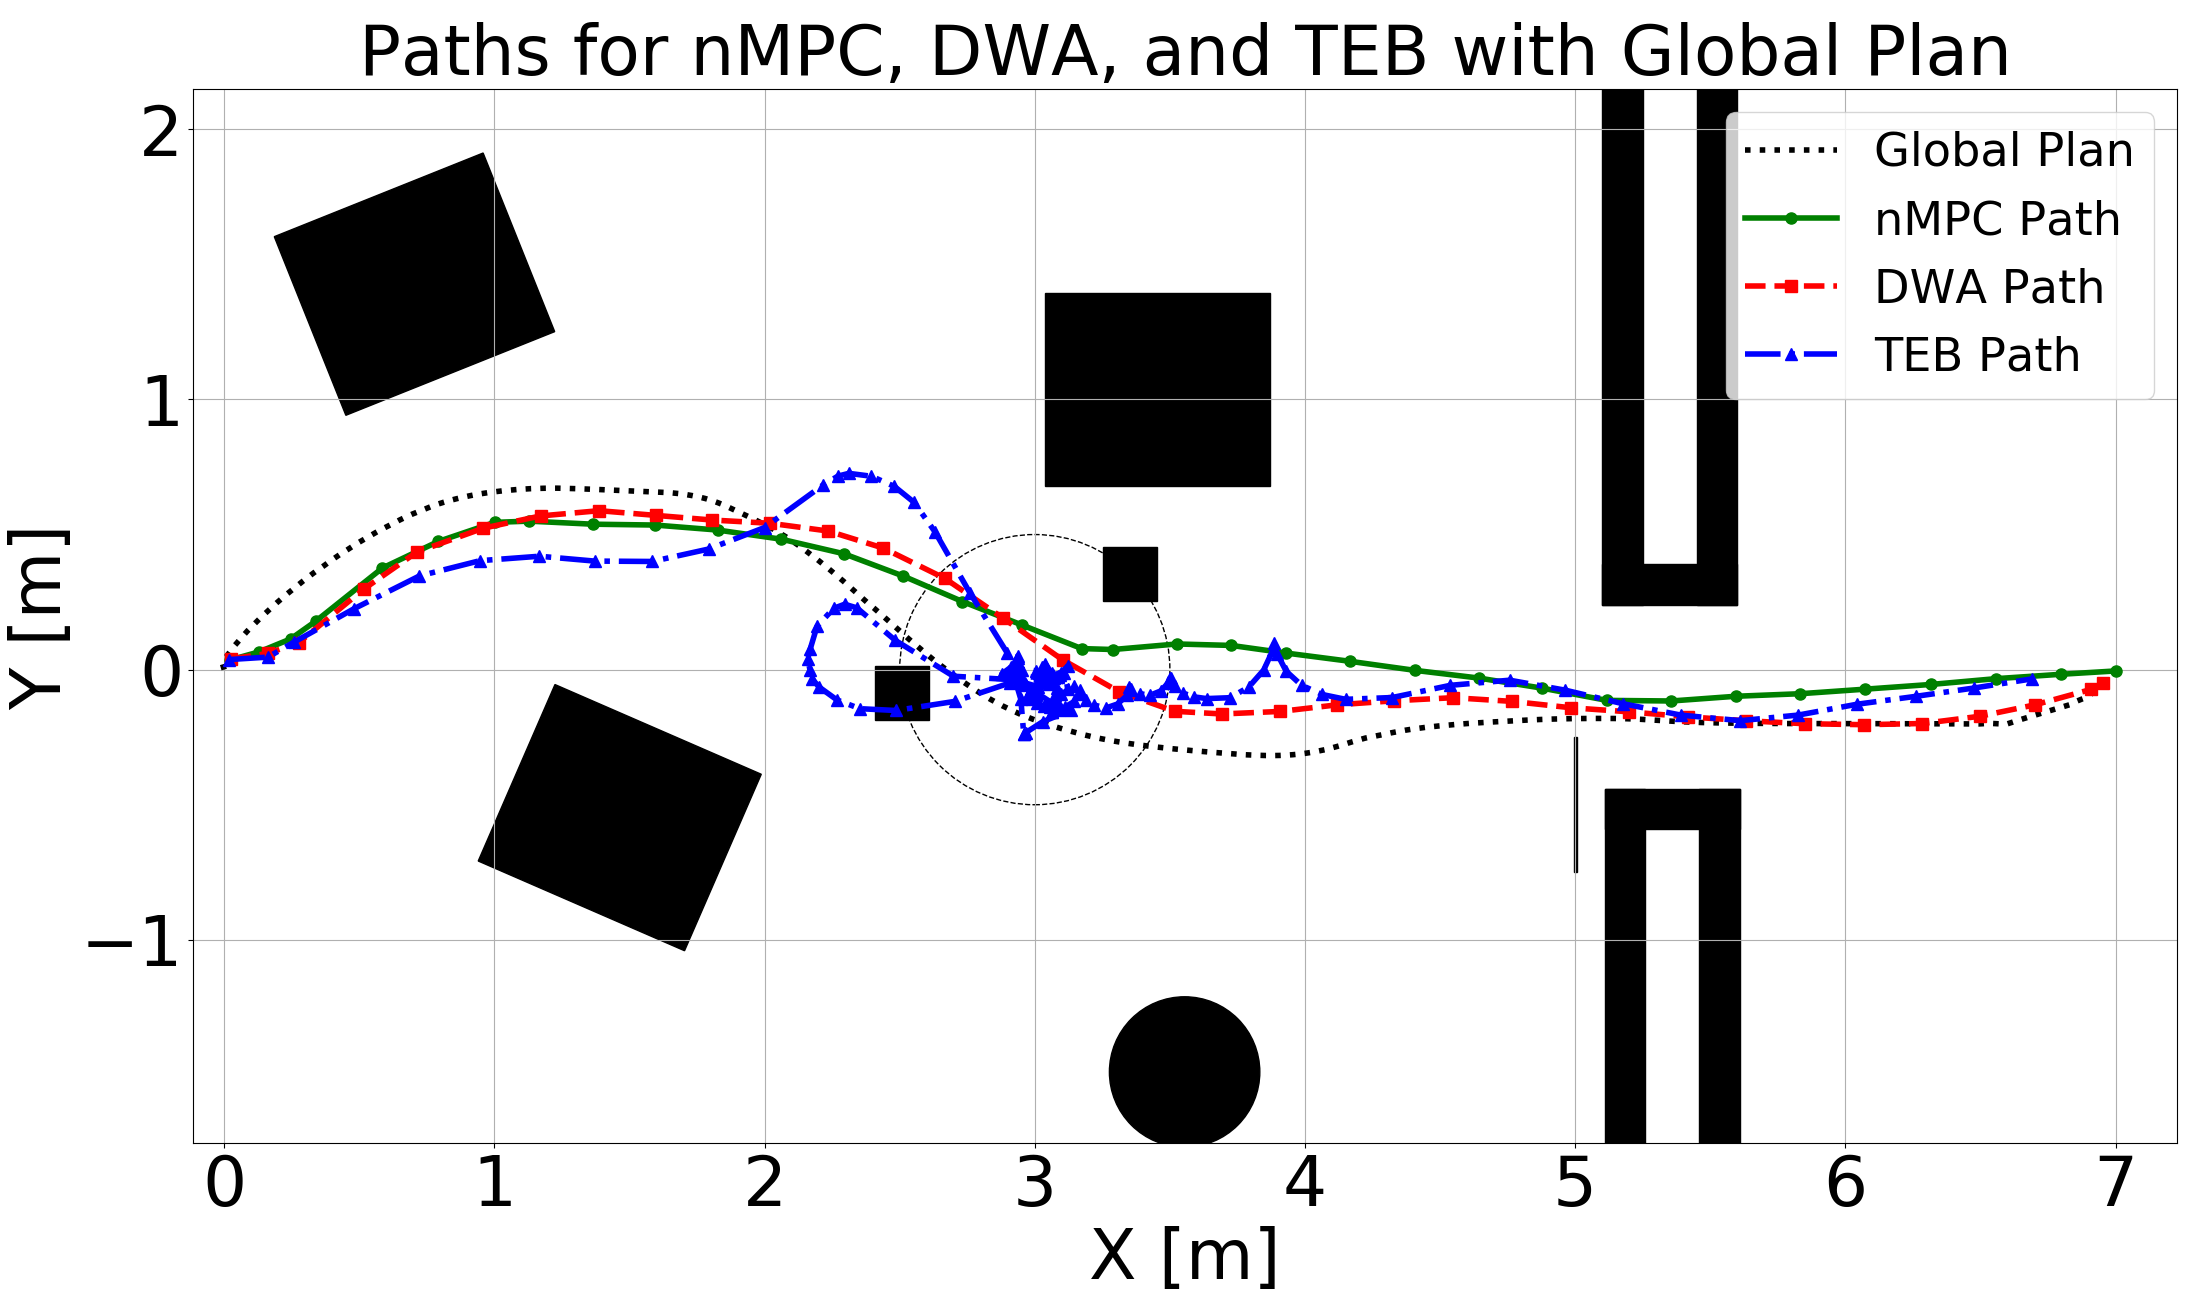
\includegraphics[width=1\columnwidth]{images/nMPC_15_vs_DWA_10_vs_TEB_8_Path.png}
    \caption{ }
    \label{fig:nMPC_16_vs_DWA_12_vs_TEB_6_Path}
\end{figure}

\begin{figure}[!h]
    \centering
    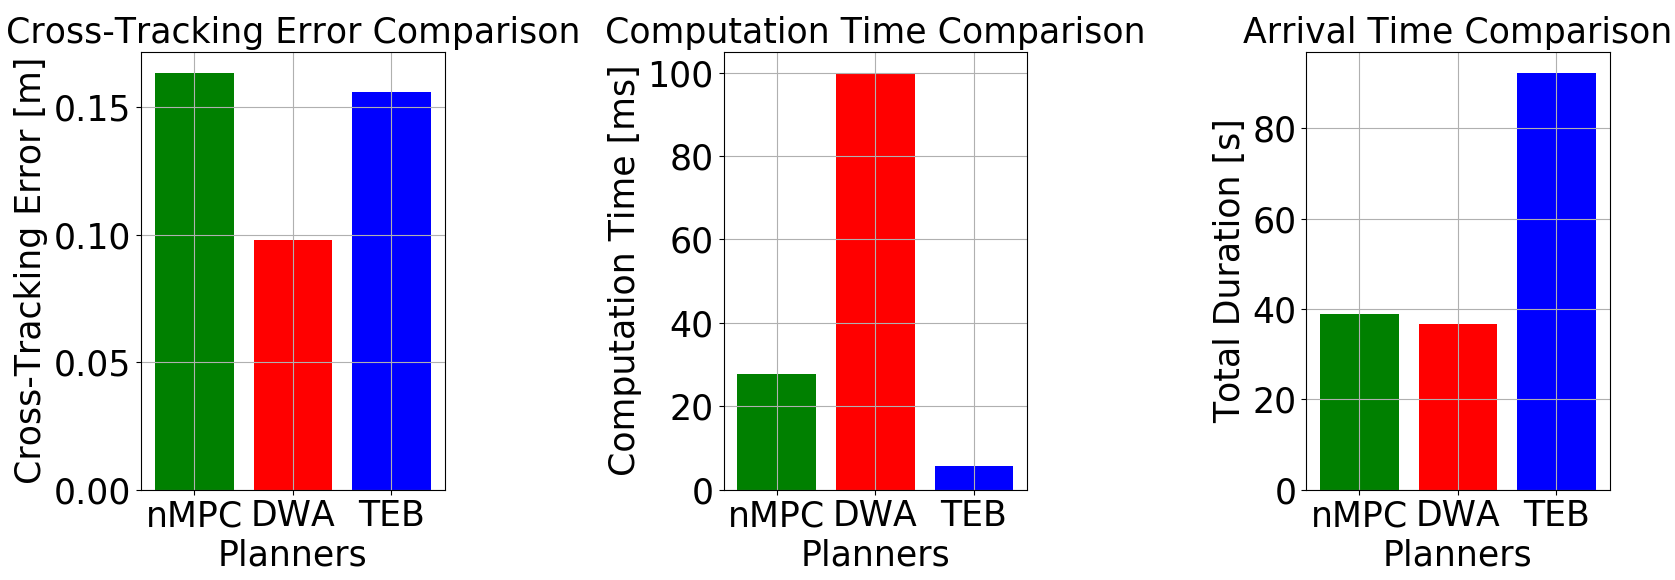
\includegraphics[width=1\columnwidth]{images/nMPC_15_vs_DWA_10_vs_TEB_8.png}
    \caption{ }
    \label{fig:nMPC_16_vs_DWA_12_vs_TEB_6_Path}
\end{figure}

\begin{figure}[!h]
    \centering
    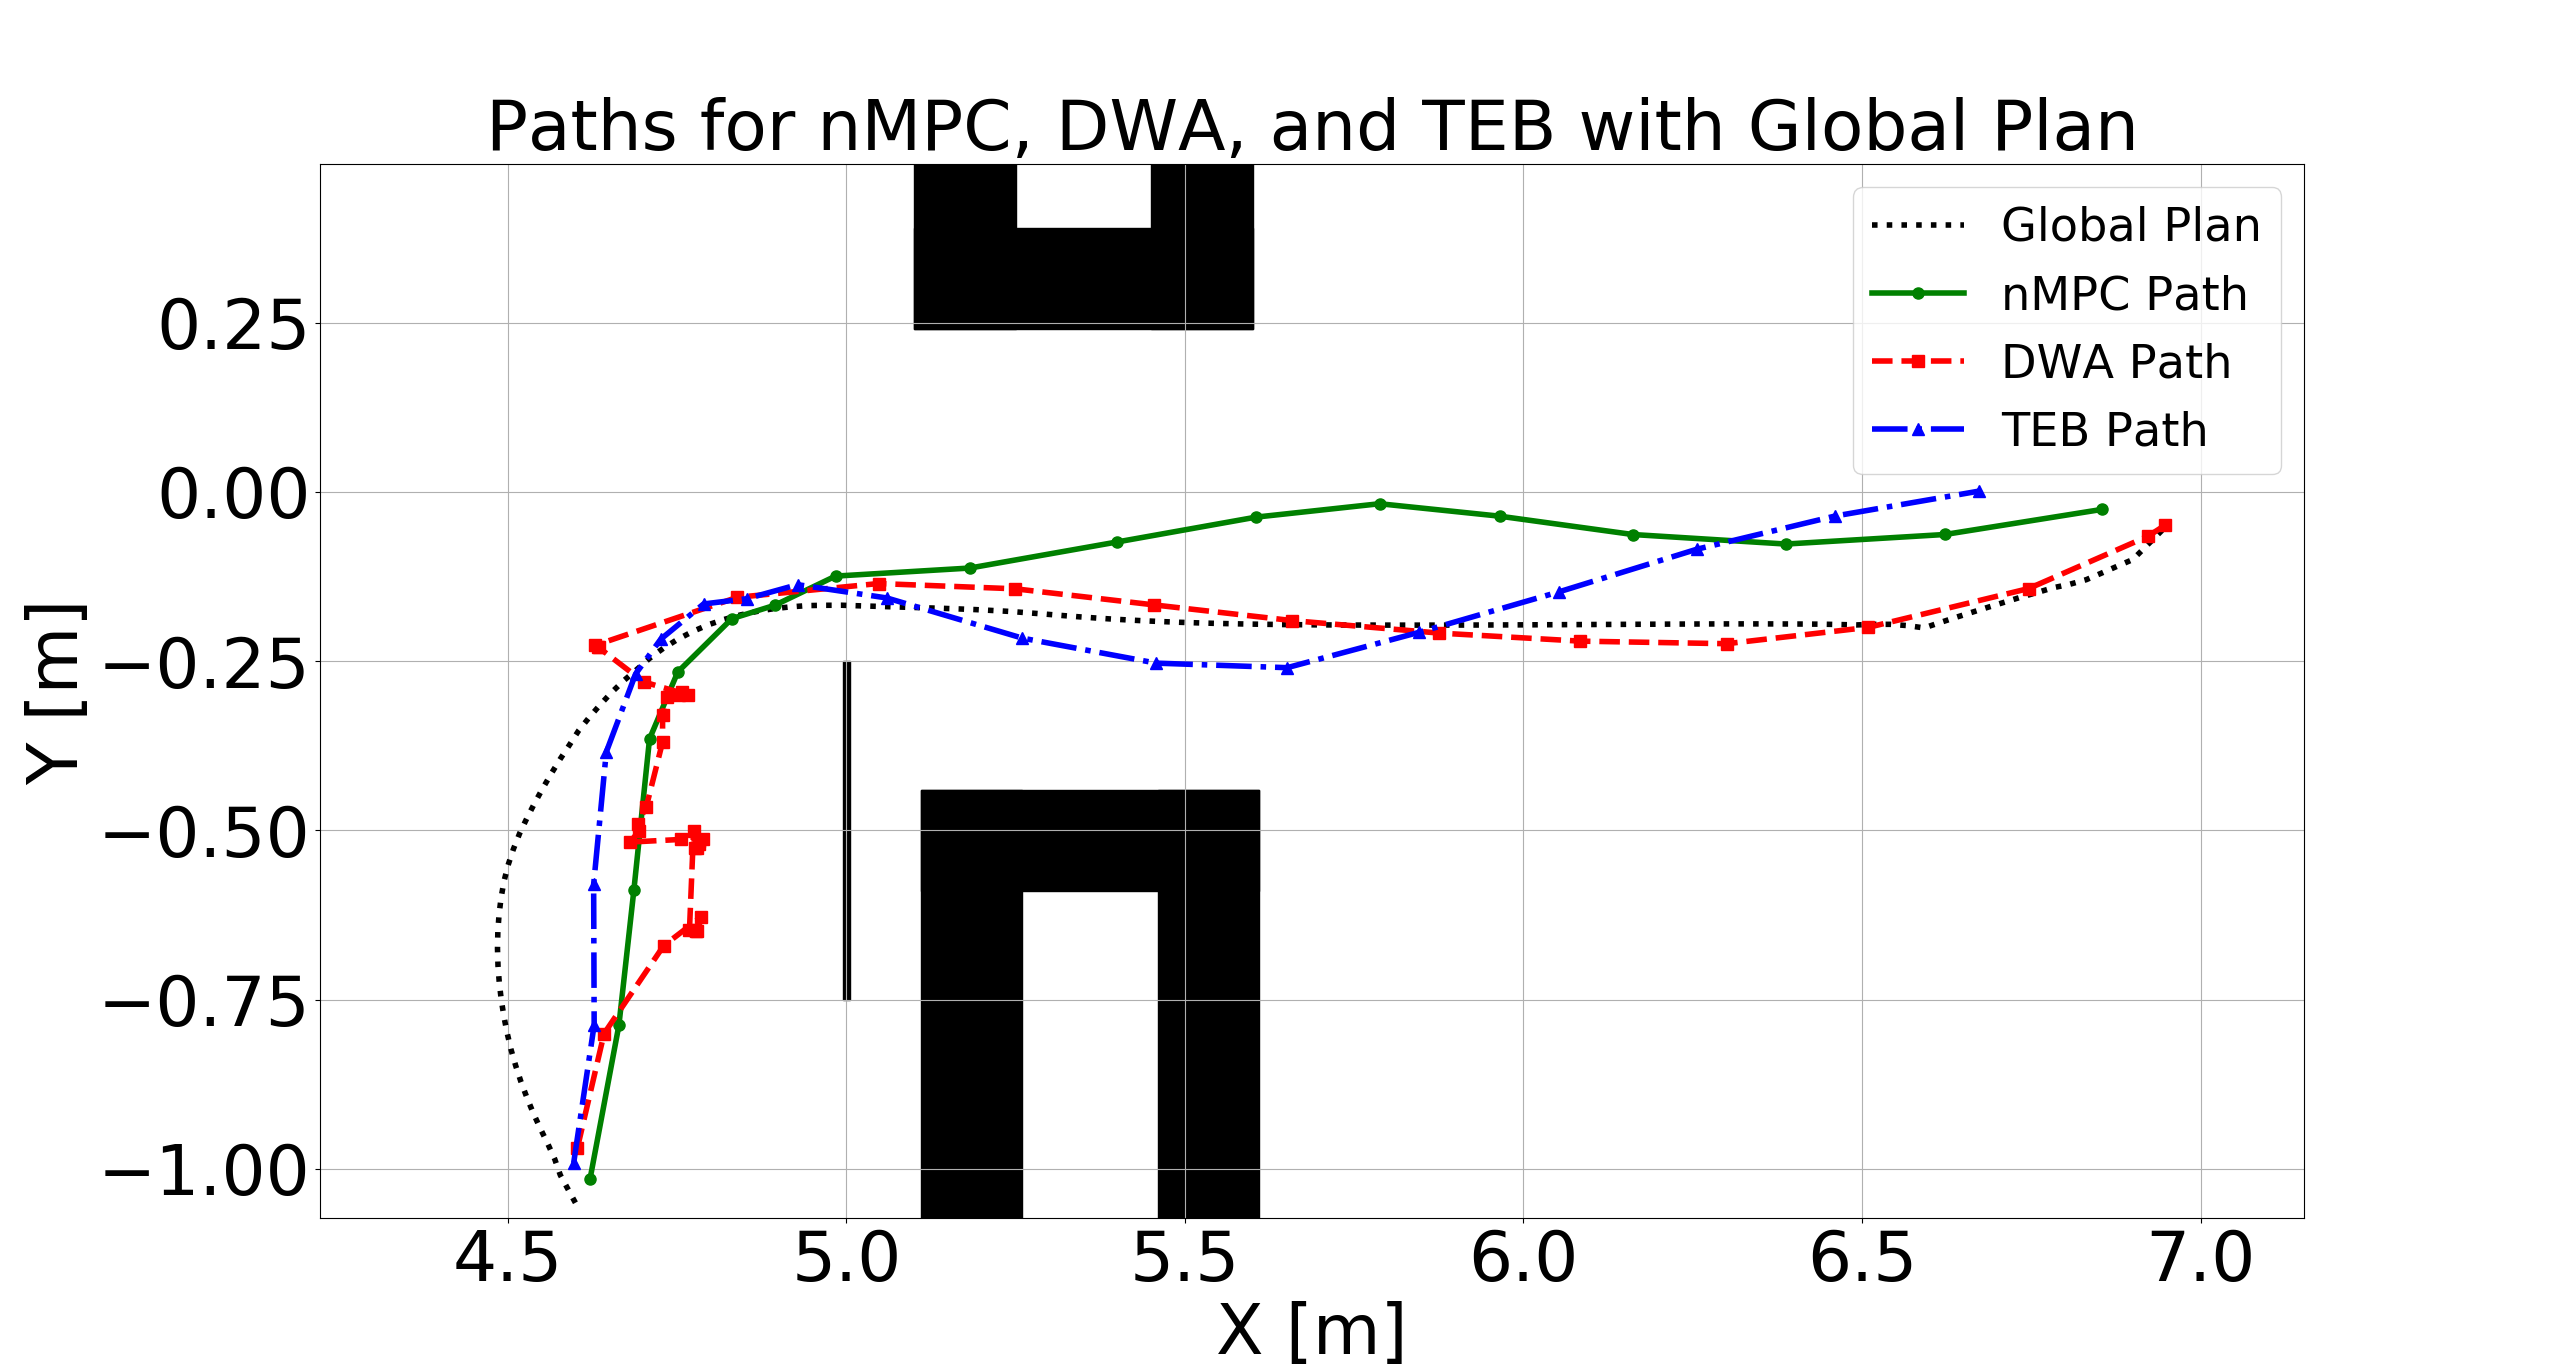
\includegraphics[width=1\columnwidth]{images/nMPC_16_vs_DWA_12_vs_TEB_9_Path.png}
    \caption{ }
    \label{fig:nMPC_16_vs_DWA_12_vs_TEB_6_Path}
\end{figure}

\begin{figure}[!h]
    \centering
    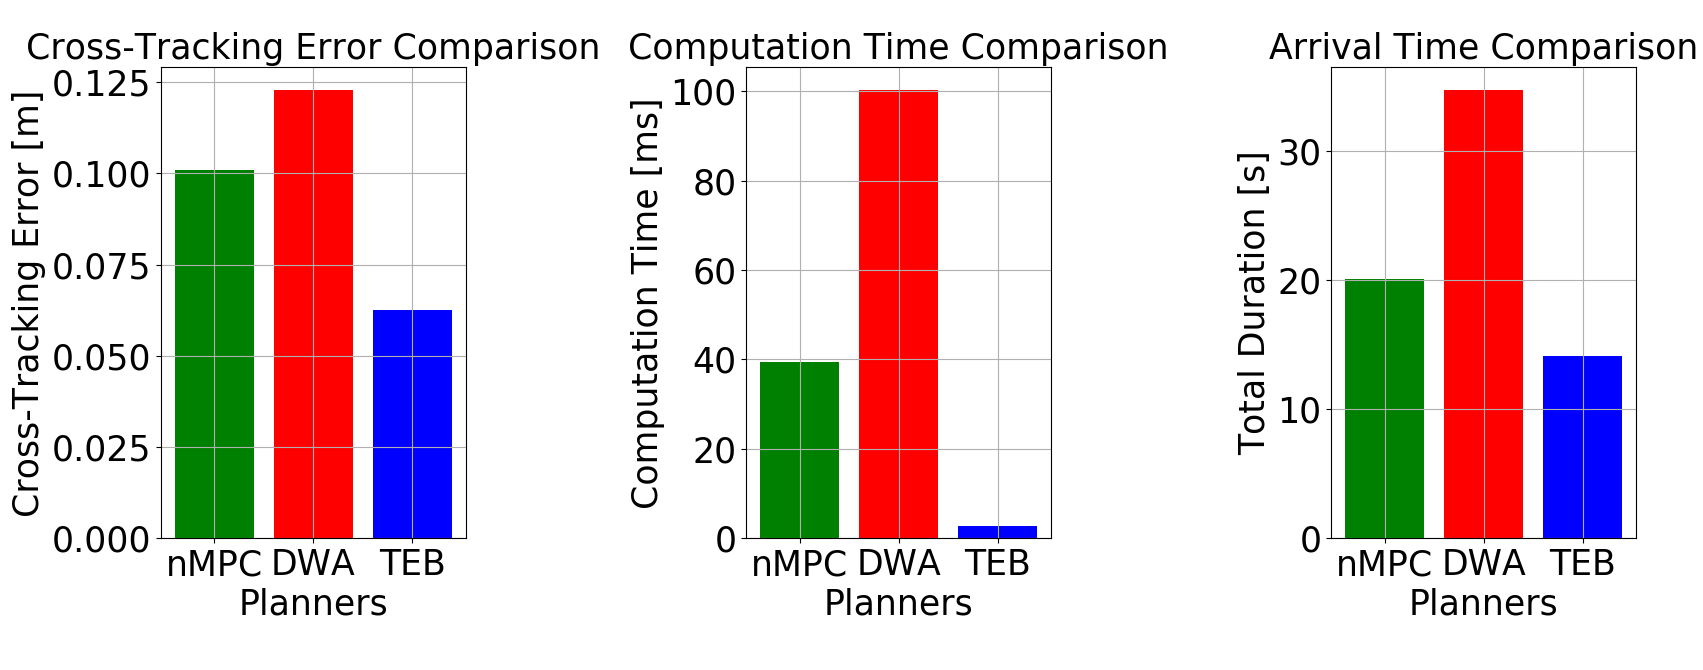
\includegraphics[width=1\columnwidth]{images/nMPC_16_vs_DWA_12_vs_TEB_9.png}
    \caption{ }
    \label{fig:nMPC_16_vs_DWA_12_vs_TEB_6_Path}
\end{figure}


\begin{figure}[!h]
    \centering
    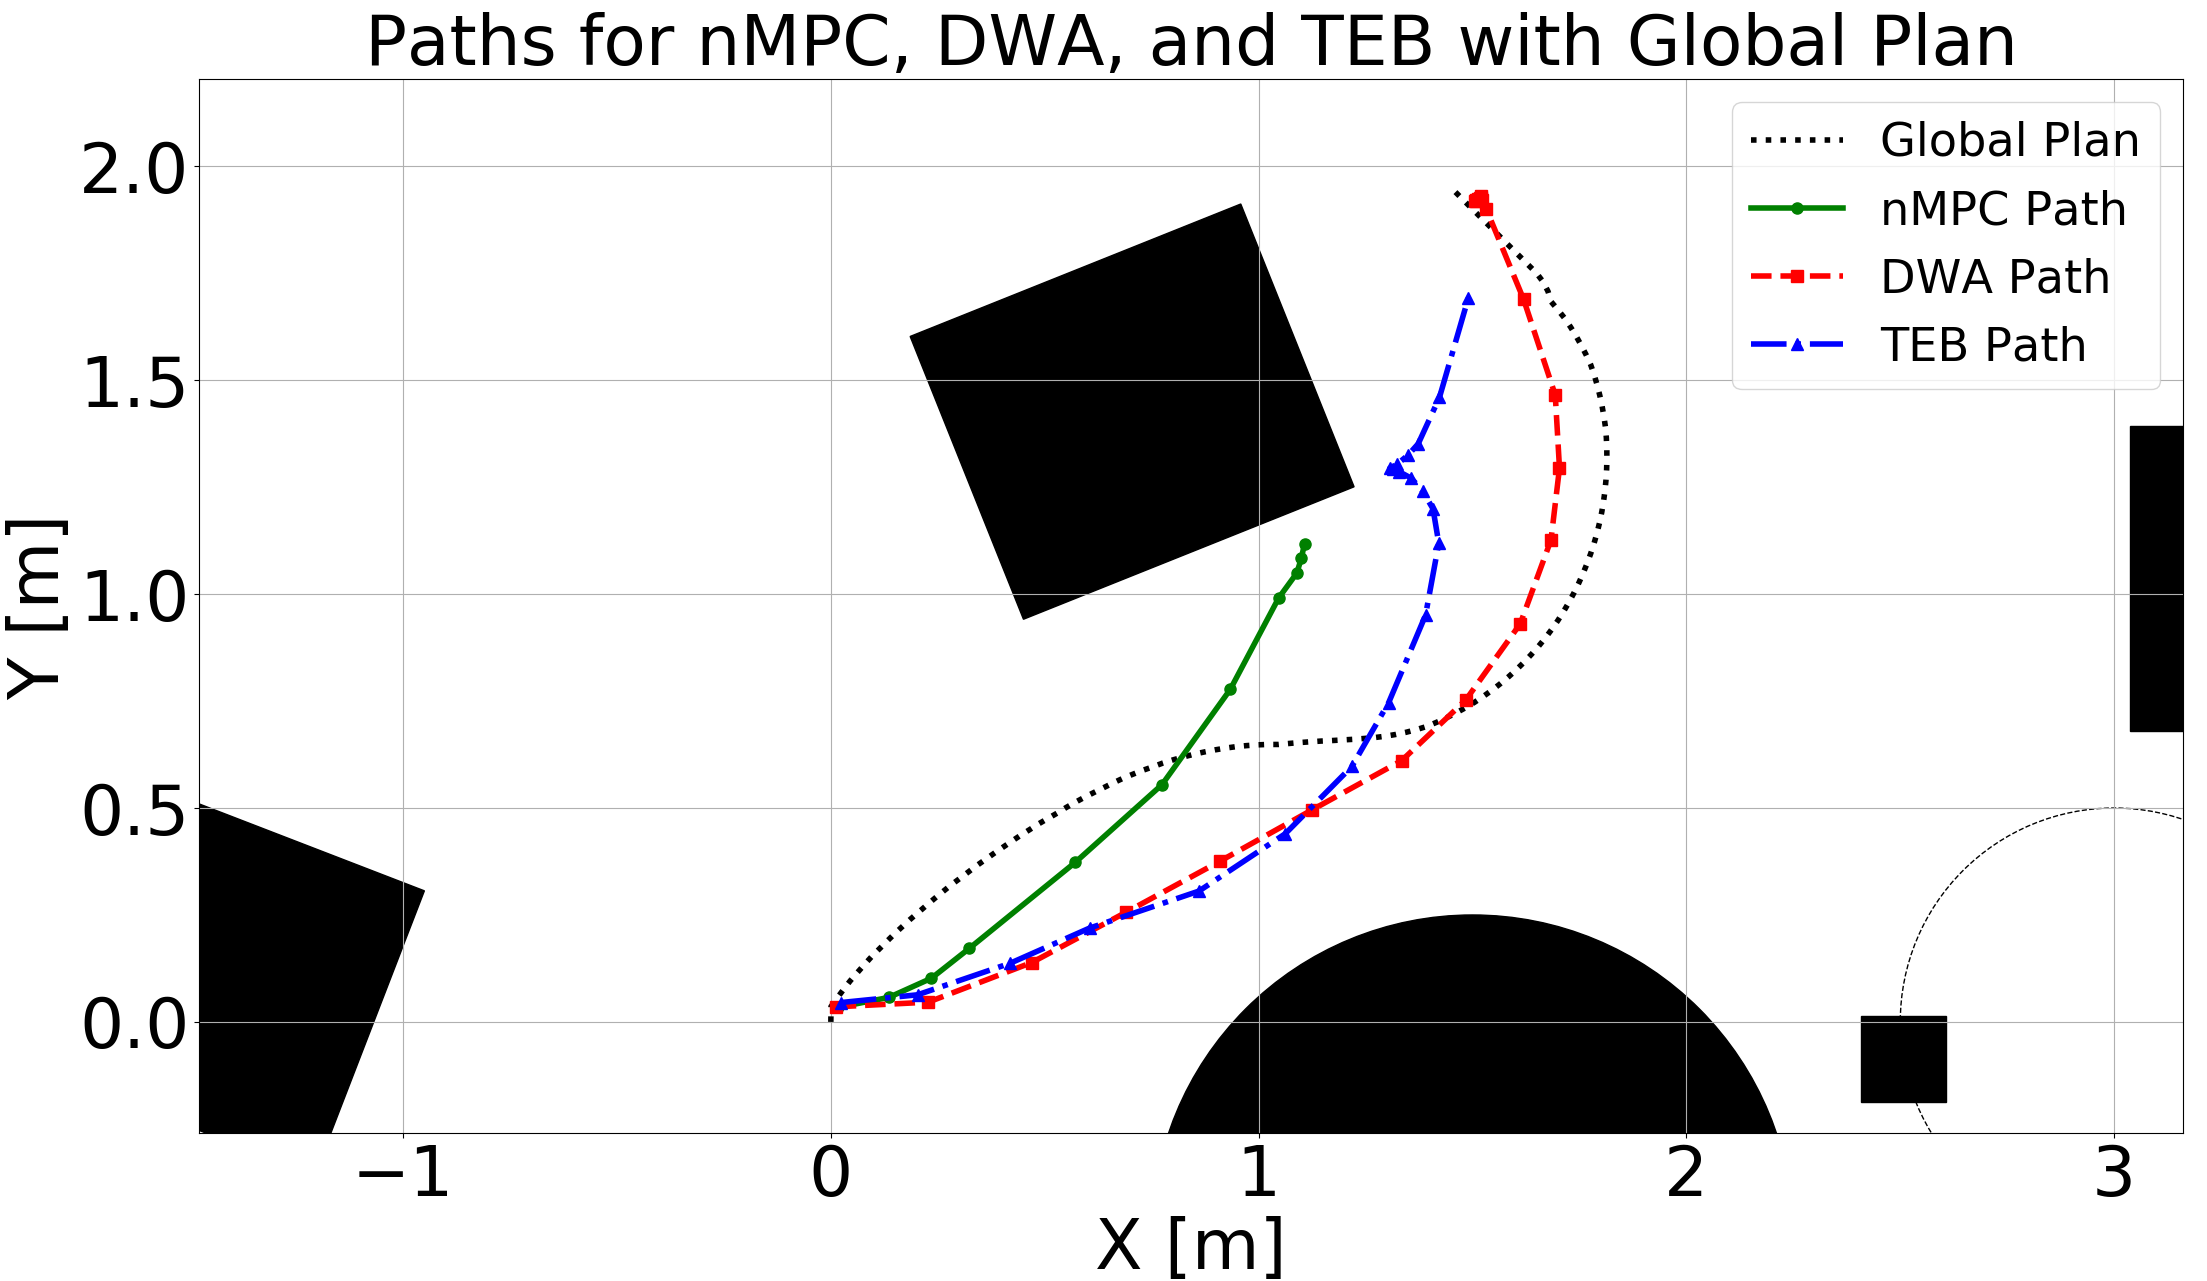
\includegraphics[width=1\columnwidth]{images/nMPC_18_vs_DWA_15_vs_TEB_10_Path.png}
    \caption{ }
    \label{fig:nMPC_16_vs_DWA_12_vs_TEB_6_Path}
\end{figure}

\begin{figure}[!h]
    \centering
    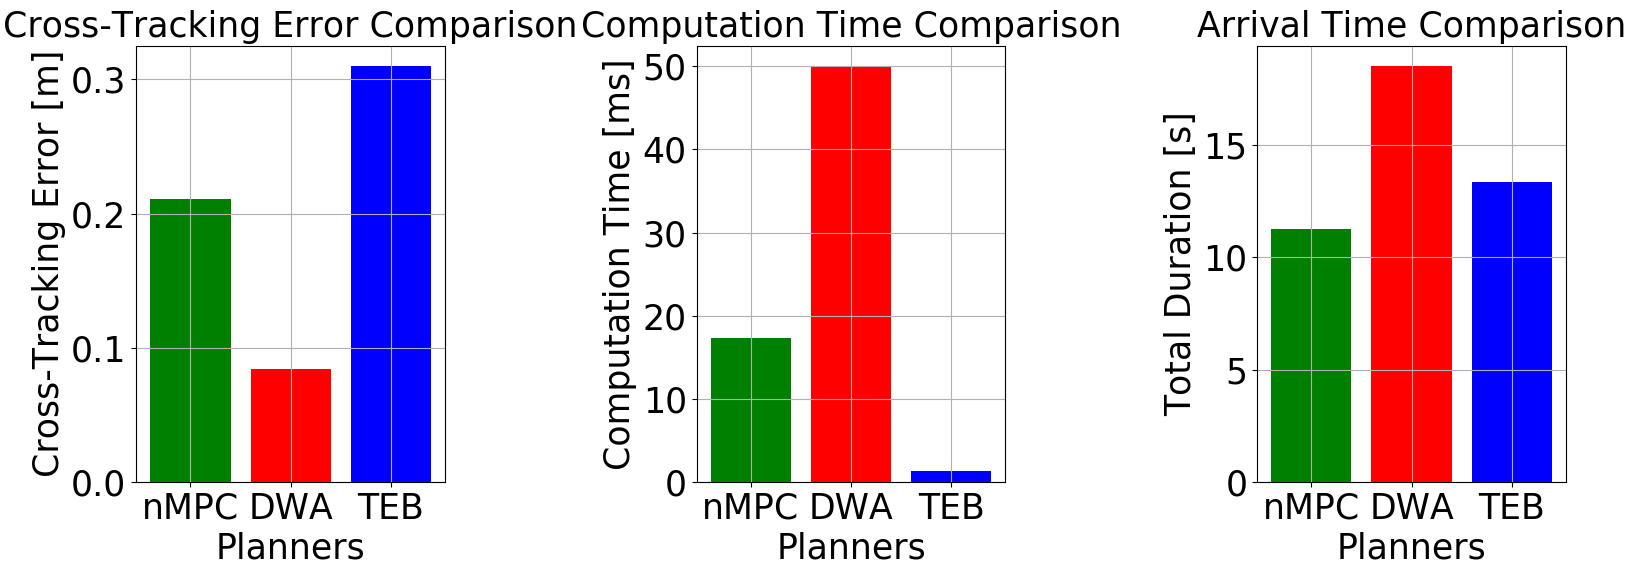
\includegraphics[width=1\columnwidth]{images/nMPC_18_vs_DWA_15_vs_TEB_10.png}
    \caption{ }
    \label{fig:nMPC_16_vs_DWA_12_vs_TEB_6_Path}
\end{figure}


%%%%%%%%%%%%%%%%%%%%%%%%%%%%%%%%%%%%%%%%%%%%%%%%%%%%%%%%%%%%%%%%%%
\section{Summary and Outlook}



%%%%%%%%%%%%%%%%%%%%%%%%%%%%%%%%%%%%%%%%%%%%%%%%%%%%%%%%%%%%%%%%%%
% Literaturverzeichnis
{\small
\bibliographystyle{IEEEtran}
\bibliography{IEEEabrv,refs}
}


%%%%%%%%%%%%%%%%%%%%%%%%%%%%%%%%%%%%%%%%%%%%%%%%%%%%%%%%%%%%%%%%%%
% End of page 3
\clearpage 

\end{document}